\colorlet{shadecolor}{\chapterColor}
\chapter{The Garden Main}\label{a:The Garden Main}
\markboth{\color{white}The Garden Main \protect\thepage \hspace{4pt}}{}
\lhead{\textcolor{\chapterColor}{\rule[-2pt]{\textwidth}{15pt}}}
\qrcode{./maps/qr/The Garden Main_qr.png}{http://maps.google.com/maps?q=44.44076010641458,-122.5752659013521}{Navigate to this area}
Located about 3.5 miles down quatzville road from highway 20, park in the Gravel pull out where the road bends left just before you reach the boulders. The Garden Main bouldering area is true to its name. A lush green space features moss covered boulders situated under a dense canopy.
\begin{figure}[h]
  \centering
    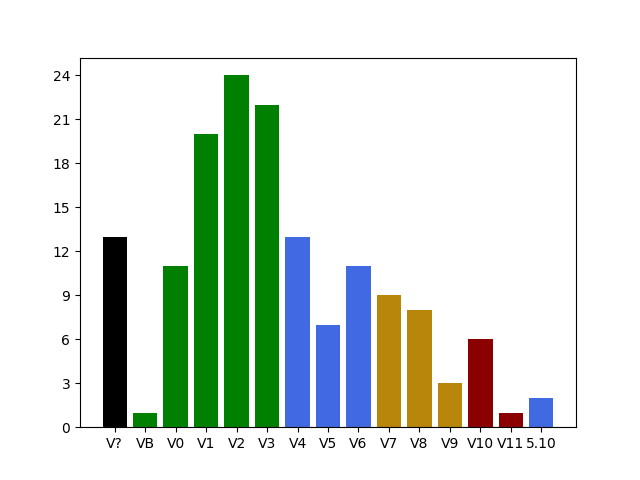
\includegraphics[width=\linewidth]{./maps/plots/The Garden Main.png}
\end{figure}

\section{Entrance Area}\label{sa:Entrance Area}
A cluster of boulders situated inbetween the two main trails.
\subsection*{Turtle Shell Boulder}\label{bf:Turtle Shell Boulder}
A short boulder with a low angle offwidth crack. If approaching on the fight club trail this is the first boulder that you will encounter

\begin{enumerate}[]
	\item\label{rt:Raphael Crack} \colorbox{green!20}{\textbf{Raphael Crack V0  } }
	\newline PLACEHOLDER\
\end{enumerate}
\subsection*{Toilet Bowl}\label{bf:Toilet Bowl}
If approaching via the main trail this is the first boulder you will encounter just of the road.

\begin{enumerate}[resume]
	\item\label{rt:Toilet Bowl} \colorbox{green!20}{\textbf{Toilet Bowl V1  } }
	\newline PLACEHOLDER\
	\item\label{rt:Scrubbing Bubbles} \colorbox{green!20}{\textbf{Scrubbing Bubbles V1  } }
	\newline PLACEHOLDER\
\end{enumerate}
\subsection*{Boys In the Woods}\label{bf:Boys In the Woods}
A low boulder with an identifiable scoop on the downhill side is located on the main trail roughly 150ft uphill from the road.

\begin{enumerate}[resume]
	\item\label{rt:Boys in the Woods} \colorbox{RoyalBlue!20}{\textbf{Boys in the Woods V4 \ding{72} \ding{72}  } }
	\newline Start on a low jug just before the scoop at the lowest part of the boulder. Climb up the left arete of the scoop until you can flop in. Some may consider this an eliminate since, with difficulty, you could also just mantle directly into the scoop.\
	\item\label{rt:Cuba Gooding} \colorbox{RoyalBlue!20}{\textbf{Cuba Gooding V5  } }
	\newline Start as for Boys in the Woods but climb right along the lip of the scoop until you can reach the holds at the top of Ice Cubes Shiny Jerry Curl\
	\item\label{rt:Ice Cubes Shiny Jerry Curl} \colorbox{RoyalBlue!20}{\textbf{Ice Cubes Shiny Jerry Curl V6  } }
	\newline Start on a low sloping edge and pull some sneaky moves to gain a knife edge crimp at eye level. Continue straight up.\
\end{enumerate}
\subsection*{Tree Slab}\label{bf:Tree Slab}
A narrow slab just uphill and to the right of the Boys in the Woods boulder.

\begin{enumerate}[resume]
	\item\label{rt:Tree Slab} \colorbox{green!20}{\textbf{Tree Slab V1 \ding{72} \ding{72}  } }
	\newline Climb the center of the slab.\
\end{enumerate}
\subsection*{All Sorts of Ease}\label{bf:All Sorts of Ease}
A low angle slab under the Meth Lab prow

\subsection*{Tonsil}\label{bf:Tonsil}
A small hanging boulder under the Meth Lab prow.

\subsection*{Three Star Ledge}\label{bf:Three Star Ledge}
Angular boulder in the rocky landscape between the two entrance trails.

\section{Fight Club}\label{sa:Fight Club}
Located in the southwest corner of the Garden main, The Fight Club zone is home to the namesake V8 test piece as well as several other quality lines. Flat landings and easy access make this a nice spot to spend some time
\halfPic{}{./maps/subarea/fightClub_c.png}{Fight Club Area Map}
\halfPic{}{./maps/subarea/undertow_c.png}{Undertow area map}
\subsection*{The Office}\label{bf:The Office}
A tall not quite vertical boulder is immediately on your right as you enter the Fight Club Area

\begin{enumerate}[]
	\item\label{rt:Jim Halpert} \colorbox{green!20}{\textbf{Jim Halpert V1 \ding{73} \warn \warn } }
	\newline Starting on the right edge of the block climb climb the right corner over a rocky landing. Either pull some harder moves to stay on the downhill face or round the corner to the right and pull some easier moves over a worse landing. Grade and rating unconfirmed.\
	\item\label{rt:Daryl Philbin} \colorbox{green!20}{\textbf{Daryl Philbin V1 \ding{72} \ding{72} \ding{72}  \warn } }
	\newline Starting at the Center of the block climb left on good holds to the arete. Climb up the arete until you can reach good face holds up right and continue through a, thankfully, juggy top out. Mind the rock at the base of the climb. Left and right alternative starts add a little variety but do not change the grade.\
\end{enumerate}
\subsection*{Crash Test Dummies}\label{bf:Crash Test Dummies}
A small boulder in between The Office and Fight Club.

\begin{enumerate}[resume]
	\item\label{rt:Vince} \colorbox{green!20}{\textbf{Vince V2 \ding{72} \ding{72}  } }
	\newline Squat start on good edges. Navigate a crescent shaped sidpull rail to a delicate top out. Make sure to clean the top out before attempting.\
\end{enumerate}
\subsection*{Fight Club}\label{bf:Fight Club}
The obvious overhanging boulder with an interesting bubbly texture.

\halfPic{ (See Page \pageref{rt:Fight Club})}{./images/FightClub2.jpg}{Michael near the top of Fight Club.}\label{pt:Fight Club}
\begin{enumerate}[resume]
	\item\label{rt:The Ear} \colorbox{green!20}{\textbf{The Ear V2 \ding{72} \ding{72} \ding{72}  } }
	\newline Start on the arete at the far right end of the boulder. Climb straight up through tricky holds to a heady top out.\
	\item\label{rt:Fight Club} \colorbox{Goldenrod!50}{\textbf{Fight Club V8 \ding{72} \ding{72} \ding{72}  } }
	\newline Area classic, this rig is a feather in any would be crushers cap. Start on the far right arete as for Ear. Traverse across the angle change and top out above a bubbly crimp rail on the overhanging face.\
	\item\label{rt:Fight Club Left} \colorbox{black!20}{\textbf{Fight Club Left V?  } }
	\newline PLACEHOLDER\
\end{enumerate}
\subsection*{Tyler Durten}\label{bf:Tyler Durten}
Just to the left of the fight club boulder is a tall wall with few features other than a distinctive crimp rail at eye level.

\begin{enumerate}[resume]
	\item\label{rt:Tyler Durten} \colorbox{green!20}{\textbf{Tyler Durten V3 \ding{72}  } }
	\newline Start on a henious crimp rail and punch out left to much better holds.\
	\newline \textbf{Variations:}
	\begin{enumerate}
		\item\label{vr:Tyler Durten Dyno} \colorbox{black!20}{\emph{Tyler Durten Dyno V?  }  }
		\newline It has been speculated that the dyno from the starting hold straight to the lip will go.\
	\end{enumerate}
\end{enumerate}
\fullPic{}{./maps/topos/miniMe2_c.png}{Routes on Mini Me, Trust, and Tyler Durten}
\subsection*{Mini Me}\label{bf:Mini Me}
A short pointy boulder with a flat landing is nearly freestanding on the downhill side of the Fight Club zone

\begin{enumerate}[resume]
	\item\label{rt:Mini Me} \colorbox{green!20}{\textbf{Mini Me V3 \ding{73} } }
	\newline start on blunt corner. Make tricky moves to a blocky jug to the lip and traverse left to an easy top over a rocky landing\
	\item\label{rt:Austin Powers} \colorbox{RoyalBlue!20}{\textbf{Austin Powers V5 \ding{72}  } }
	\newline Start as for Mini Me but move right into top of Dr. Evil\
	\item\label{rt:Dr. Evil} \colorbox{green!20}{\textbf{Dr. Evil V3 \ding{72}  } }
	\newline sit start in compression with left hand on a low sloper sidepull and right hand on the arete. Pull some tricky moves to gain better holds either rolling onto the right hand slab early or staying on the arete the whole way.\
	\newline \textbf{Variations:}
	\begin{enumerate}
		\item\label{vr:Mr. Bigglesworth} \colorbox{green!20}{\emph{Mr. Bigglesworth V1 \ding{72} \ding{72}  }  }
		\newline Start on your choice of waist high holds, climb straight up the right face or stay left on the arete. Authors note: other guides identify several other variations on this route, this book intentionally omits other variations in preference of encouraging climbers to find their own beta.\
	\end{enumerate}
\end{enumerate}
\subsection*{Trust}\label{bf:Trust}
The Trust boulder sits on an terrace behind Mini Me and to the Left of Tyler Durten

\begin{enumerate}[resume]
	\item\label{rt:Trust} \colorbox{green!20}{\textbf{Trust V2 \ding{72} \ding{72} \ding{72}  } }
	\newline Sit start in compression on a hanging refrigerator block. Climb straight up through a slopeing ledge to the top. Look for the juggy crack ~1ft inset from the lip.\
	\newline \textbf{Variations:}
	\begin{enumerate}
		\item\label{vr:Iron Cross} \colorbox{green!20}{\emph{Iron Cross V2 \ding{72}  }  }
		\newline Avoid the committing moves at the lip by traversing left early.\
	\end{enumerate}
\end{enumerate}
\subsection*{E's Dirty B}\label{bf:E's Dirty B}
Following a faint trail west traveling past the trust boulder brings you to a Large boulder which almost immediately gives way to low angle slab.

\begin{enumerate}[resume]
	\item\label{rt:E's Dirty B} \colorbox{RoyalBlue!20}{\textbf{E's Dirty B V5 \ding{72} \ding{72}  } }
	\newline Start with hands matched on a lumpy flake in the back of a small cave. Using slopeing edges out right and a difficult undercling navigate out of the cave trending right at the lip to a jug. The final slab quest is an enjoyable and easy top out.\
\end{enumerate}
\subsection*{Silly Steep}\label{bf:Silly Steep}
Thin overhanging block left of the Undertow boulder.

\begin{enumerate}[resume]
	\item\label{rt:Silly Steep Mantle} \colorbox{green!20}{\textbf{Silly Steep Mantle V1  } }
	\newline PLACEHOLDER\
\end{enumerate}
\subsection*{Undertow}\label{bf:Undertow}
Realatively off the beaten path as far as classic garden boulders goes. Follow a faint trail upill past the trust boulder.

\halfPic{ (See Page \pageref{rt:Riptide})}{./images/Riptide.jpg}{Rob on Riptide}\label{pt:Riptide}
\begin{enumerate}[resume]
	\item\label{rt:Undertow} \colorbox{green!20}{\textbf{Undertow V3 \ding{72} \ding{72} \ding{72}  } }
	\newline Start on two boob shaped slopers at head height. Climb straight up using face holds and the right arete.\
	\newline \textbf{Variations:}
	\begin{enumerate}
		\item\label{vr:Undertow Sit} \colorbox{RoyalBlue!20}{\emph{Undertow Sit V6  }  }
		\newline Sit start with left hand in a slopey dish and right hand on a low sidepull. Pull some bizzare moves to join into Undertow.\
		\item\label{vr:Undertow Sit Right} \colorbox{Goldenrod!50}{\emph{Undertow Sit Right V7 \ding{72} \ding{72} \ding{72}  }  }
		\newline Sit start in the scoop ~4ft right of Undertow sit with left hand on a borken sidepull and right hand on a low undercling, climb into undertow. At one point this line was simply refered to as Undertow, for this book modern naming standards have been conserved.\
	\end{enumerate}
	\item\label{rt:Riptide} \colorbox{green!20}{\textbf{Riptide V3 \ding{72} \ding{72}  } }
	\newline Start as for undertow but trend right around the corner to a juggy hueco top out.\
	\item\label{rt:Tidepool} \colorbox{black!20}{\textbf{Tidepool V?  } }
	\newline PLACEHOLDER\
\end{enumerate}
\section{Meth Lab}\label{sa:Meth Lab}
Easily the most recognizable feature at the Garden, the Meth Lab boulder towers over all other stones in the main area. Most climbs for this zone are located in a secluded natural amphitheater on the uphill side of the boulder.
\halfPic{}{./maps/topos/smackdown_c.png}{Meth Lab backside}
\halfPic{}{./maps/topos/octurnal_c.png}{Meth Lab backside}
\halfPic{}{./maps/topos/octurnal2_c.png}{Meth Lab across from E's}
\subsection*{Meth Lab}\label{bf:Meth Lab}
Routes listed in counter clockwise order beginning under the large prow of the downhill face.

\halfPic{ (See Page \pageref{rt:Octurnal})}{./images/Octurnal.jpg}{Carson landing the big throw on Octurnal. Classic!}\label{pt:Octurnal}
\begin{enumerate}[]
	\item\label{rt:Meth Lab Project} \colorbox{black!20}{\textbf{Meth Lab Project V?  \warn \warn \warn } }
	\newline The obvious prow on the front of the Meth Lab boulder has a bolted top rope anchor but a route up it has likely never been free'ed by any means. The ethics of climbing this behemoth are contentious but in my opion it is fair game to bolt as a sport route. If you have the desire to do so consider working it out on TR first before placing new equipment.\
	\item\label{rt:Don't Blow the Jug} \colorbox{green!20}{\textbf{Don't Blow the Jug V2  } }
	\newline Start at the base of the wide crack. Climb the offwidth until you can make use of a jug to squeeze into the crack. Walk through the crack to the far side of the boulder.\
	\item\label{rt:Trust Issues} \colorbox{Goldenrod!50}{\textbf{Trust Issues V8  \warn \warn } }
	\newline PLACEHOLDER\
	\item\label{rt:Leave It to Jesus} \colorbox{green!20}{\textbf{Leave It to Jesus V1 \ding{72} \ding{72}  } }
	\newline Stand start on a high blocky edge. Crank one move and post up for a fun huck.\
	\newline \textbf{Variations:}
	\begin{enumerate}
		\item\label{vr:Leave it to Jesus Sit} \colorbox{Goldenrod!50}{\emph{Leave it to Jesus Sit V8  }  }
		\newline PLACEHOLDER\
	\end{enumerate}
	\item\label{rt:Smackdown} \colorbox{Goldenrod!50}{\textbf{Smackdown V7 \ding{72} \ding{72}  } }
	\newline Start standing with left hand gaston and right hand jug sidepull. Crank some powerful moves on bad feet and follow the line of crimps to a top out left\
	\newline \textbf{Variations:}
	\begin{enumerate}
		\item\label{vr:Harbor Freight} \colorbox{Goldenrod!50}{\emph{Harbor Freight V8 \ding{72} \ding{72} \ding{72}  }  }
		\newline Sit down start with hands matched on a blocky undercling, climb into Smackdown. This variation was literally unearthed when a local climber yarded a large rock out from the landing of Smackdown using a chain and come along. The device broke in the process inspiring the name of the route.\
	\end{enumerate}
	\item\label{rt:Heisenburg} \colorbox{Goldenrod!50}{\textbf{Heisenburg V9  } }
	\newline PLACEHOLDER\
	\item\label{rt:Learys Lunge} \colorbox{Goldenrod!50}{\textbf{Learys Lunge V9  } }
	\newline PLACEHOLDER\
	\item\label{rt:Guillotine} \colorbox{RoyalBlue!20}{\textbf{Guillotine V4 \ding{72} \ding{72}  } }
	\newline Start underclinging on the hanging "Guillotine blade" flake left of Octurnal. Climb straight up.\
	\item\label{rt:Octurnal} \colorbox{Goldenrod!50}{\textbf{Octurnal V7 \ding{72} \ding{72} \ding{72}  } }
	\newline For many this is THE local test piece. Start sitting with left hand on a sloping triangular rib and right hand on a slopey cripm at the arete. Crank a few hard moves to gain the lip then traverse left through the lightning bolt hold to a pumpy top out. Originally known as "Tom's phsychadelic trip".\
	\newline \textbf{Variations:}
	\begin{enumerate}
		\item\label{vr:Direct Exit} \colorbox{Goldenrod!50}{\emph{Direct Exit V7 \ding{72} \ding{72} \ding{72}  }  }
		\newline Of all the Octurnal exits this one has the most interesting moves. Climb Octurnal to the ledge then pull some tricky moves to round the right arete. Continue on through a heads up top out.\
		\item\label{vr:Center Exit} \colorbox{Goldenrod!50}{\emph{Center Exit V7 \ding{72} \ding{72}  }  }
		\newline The easiest top option for this boulder involves pulling through a suprisingly good side pull above the left end of the ledge. For years this variation livided in moss covered obscurity. Climbing it will make you wonder why the awkward pumpfest traverse exit is the default line\
	\end{enumerate}
	\item\label{rt:Two Blows One Stroke} \colorbox{RoyalBlue!20}{\textbf{Two Blows One Stroke V6  } }
	\newline PLACEHOLDER\
\end{enumerate}
\halfPic{}{./maps/topos/swollen_c.png}{Swollen Member}
\subsection*{Swollen Member}\label{bf:Swollen Member}
A small prow just out of the hill side above the Meth Lab boulder protrudes at a provocative angle.

\begin{enumerate}[resume]
	\item\label{rt:Swollen Member} \colorbox{green!20}{\textbf{Swollen Member V3 \ding{72} \ding{72}  } }
	\newline A classic hazing route. Start hugging the underside of the block underside with good hand holds on each side of the stubby prow. Manuver youself into a less scandelous orientation using toe hooks, heel hooks and  all manner of dirty tricks.\
\end{enumerate}
\halfPic{}{./maps/topos/enchilada_c.png}{Enchilada}
\subsection*{E's Boulder}\label{bf:E's Boulder}
A large boulder directly to the right of Octurnal holds a few notable routes.

\begin{enumerate}[resume]
	\item\label{rt:Slam Dunk} \colorbox{Goldenrod!50}{\textbf{Slam Dunk V7  } }
	\newline PLACEHOLDER\
	\item\label{rt:E's} \colorbox{Goldenrod!50}{\textbf{E's V7  } }
	\newline PLACEHOLDER\
	\item\label{rt:Enchilada} \colorbox{Goldenrod!50}{\textbf{Enchilada V9 \ding{72} \ding{72}  } }
	\newline Start matched on a good flat rail low to the ground with some awkward feet options. Cross into a comfortable crimp and fire up left before coming back right to a flat jug. Pretty classic as far as low balls go!\
\end{enumerate}
\subsection*{The Bubbler}\label{bf:The Bubbler}
A small unassuming block sits just downhill of E's boulder.

\section{Big}\label{sa:Big}
\
\subsection*{Bitchin Corners}\label{bf:Bitchin Corners}
A neet angular face sits on the downhill of an otherwise unremarkable boulder.

\begin{enumerate}[]
	\item\label{rt:Bitchin Corners} \colorbox{green!20}{\textbf{Bitchin Corners V2  } }
	\newline PLACEHOLDER\
	\newline \textbf{Variations:}
	\begin{enumerate}
		\item\label{vr:Bitchin Corners Sit} \colorbox{RoyalBlue!20}{\emph{Bitchin Corners Sit V6  }  }
		\newline PLACEHOLDER\
	\end{enumerate}
\end{enumerate}
\subsection*{Big}\label{bf:Big}
The "Big" boulder is a large moss covered boulder on the eastern boundary of the Garden Main area, in other guides this has also been called "roadside", and "North Block"

\begin{enumerate}[resume]
	\item\label{rt:All Bernd Up} \colorbox{red!20}{\textbf{All Bernd Up V10  } }
	\newline PLACEHOLDER\
\end{enumerate}
\subsection*{Hueco Wabo}\label{bf:Hueco Wabo}
An aesthetic boulder sits well off the beaten path

\begin{enumerate}[resume]
	\item\label{rt:Hueco Wabo} \colorbox{green!20}{\textbf{Hueco Wabo V3  } }
	\newline PLACEHOLDER\
\end{enumerate}
\subsection*{Baldo}\label{bf:Baldo}
\

\begin{enumerate}[resume]
	\item\label{rt:Front Side Baldo} \colorbox{green!20}{\textbf{Front Side Baldo V1  } }
	\newline PLACEHOLDER\
\end{enumerate}
\section{Azain}\label{sa:Azain}
Azain is a jumbled collection of rocks which forms the highest point of the Garden main.
\subsection*{The Good}\label{bf:The Good}
Continuing up the main trail from Boys in the Woods leads to a good boulder with two routes on the downhill face.

\begin{enumerate}[]
	\item\label{rt:The Good} \colorbox{green!20}{\textbf{The Good V3 \ding{72} \ding{72}  } }
	\newline Start matched on a juggy flake on the right side of the boulder's downhill face.\
	\item\label{rt:Another} \colorbox{green!20}{\textbf{Another V3 \ding{72}  \warn } }
	\newline start with opposing sidepulls on the center of the boulder's downhill face. Traverse to the left arete and ascend using delecate feet and unideal hands. Mind the uneven landing.\
\end{enumerate}
\subsection*{Next to The Good}\label{bf:Next to The Good}
A slender boulder hangs off the ground to the left of the Good.

\begin{enumerate}[resume]
	\item\label{rt:Next To the Good} \colorbox{green!20}{\textbf{Next To the Good V3  \warn } }
	\newline PLACEHOLDER\
\end{enumerate}
\halfPic{}{./maps/topos/nightcrawler_c.png}{Night Crawler}
\subsection*{Night Crawler}\label{bf:Night Crawler}
This iconic double arete boulder hangs like a throne near the top of the Azain formation.

\begin{enumerate}[resume]
	\item\label{rt:Night Crawler} \colorbox{red!20}{\textbf{Night Crawler V10  } }
	\newline PLACEHOLDER\
\end{enumerate}
\subsection*{Azain Front Side}\label{bf:Azain Front Side}
The tall walls of the Azain front side are located just off the main trail behind The Good.

\halfPic{ (See Page \pageref{rt:Ground Up Blowie})}{./images/blowie.jpg}{Andrew strugling to finde a finger lock on Ground up Blowie}\label{pt:Ground up Blowie}
\begin{enumerate}[resume]
	\item\label{rt:Ground Up Blowie} \colorbox{RoyalBlue!20}{\textbf{Ground Up Blowie V5 \ding{72} \ding{72}  } }
	\newline Start at the base of a diagonal finger crack. Follow the crack around a dabby tree and onto an easy slab. This route was named as an omage to the first ascent when the top out was cleaned via leafblower from a stance mid route.\
	\item\label{rt:Into the Light} \colorbox{RoyalBlue!20}{\textbf{Into the Light V6  } }
	\newline PLACEHOLDER\
	\newline \textbf{Variations:}
	\begin{enumerate}
		\item\label{vr:Into the Light Sit} \colorbox{Goldenrod!50}{\emph{Into the Light Sit V9  }  }
		\newline PLACEHOLDER\
	\end{enumerate}
	\item\label{rt:Azain Crack} \colorbox{black!20}{\textbf{Azain Crack V?  } }
	\newline PLACEHOLDER\
\end{enumerate}
\halfPic{}{./maps/topos/arboretum_c.png}{Routes on the Azain Backside}
\halfPic{}{./maps/topos/siren_c.png}{The Siren}
\subsection*{Azain Back Side}\label{bf:Azain Back Side}
Continuing up the main trail will bring you between the Azain and Big Fred boulders to the Azain backside.

\begin{enumerate}[resume]
	\item\label{rt:Locksmith} \colorbox{RoyalBlue!20}{\textbf{Locksmith V4 \ding{72} \ding{72} \ding{72}  \warn \warn } }
	\newline Also known as Hula. Sit start with a juggy left hand sidebpull and right hand on an undercling edge. Pull a few crimpy moves until you can reach a good hold on the arete. Rock over onto the slab and quest to the top. Be sure to clean the upper section before attempting this rig.\
	\newline \textbf{Variations:}
	\begin{enumerate}
		\item\label{vr:Brain Haemorrhage} \colorbox{Goldenrod!50}{\emph{Brain Haemorrhage V7  }  }
		\newline Start as for locksmith and traverse right into philanthropy\
	\end{enumerate}
	\item\label{rt:Philanthropy} \colorbox{RoyalBlue!20}{\textbf{Philanthropy V4  } }
	\newline PLACEHOLDER\
	\item\label{rt:Full Stokes} \colorbox{green!20}{\textbf{Full Stokes V2  } }
	\newline PLACEHOLDER\
	\item\label{rt:Garden Project} \colorbox{black!20}{\textbf{Garden Project V?  } }
	\newline Project. Sit start at the base of the low roof and climb into garden variety or Full Stokes. Once climbed this will be one of the hardes routes in Oregon.\
	\item\label{rt:Garden Variety} \colorbox{Goldenrod!50}{\textbf{Garden Variety V7  } }
	\newline PLACEHOLDER\
	\item\label{rt:The Arboretum} \colorbox{red!20}{\textbf{The Arboretum V11  } }
	\newline PLACEHOLDER\
	\item\label{rt:The Other Bernd} \colorbox{red!20}{\textbf{The Other Bernd V10  } }
	\newline PLACEHOLDER\
	\item\label{rt:The Siren} \colorbox{RoyalBlue!20}{\textbf{The Siren V5 \ding{72} \ding{72} \ding{72}  } }
	\newline Sit start at the base of the prow with one hand on an incut ledge and the other on the slopey rib below. Climb the prow using a few different beta options. This route is also refered to as "Witch Hunt".\
	\newline \textbf{Variations:}
	\begin{enumerate}
		\item\label{vr:The Siren Stand Start} \colorbox{green!20}{\emph{The Siren Stand Start V3 \ding{72} \ding{72}  }  }
		\newline Start with your left hand on the left arete and right hand on a good sidepull just above the sit start holds.\
	\end{enumerate}
	\item\label{rt:Gumby Arete} \colorbox{green!20}{\textbf{Gumby Arete V2 \ding{72} \ding{72}  } }
	\newline Stand start on underclings at the left side of the face. Challenge yourself by staying on the Arete the whole way up or bail onto the ledge out right and top as for Gumby Slab.\
	\item\label{rt:Gumby Slab} \colorbox{green!20}{\textbf{Gumby Slab V1 \ding{72} \ding{72} \ding{72}  } }
	\newline Stand start in the center of the face. This can be scary if not used to climbing outdoors.\
	\newline \textbf{Variations:}
	\begin{enumerate}
		\item\label{vr:Bag of Tricks} \colorbox{green!20}{\emph{Bag of Tricks V3 \ding{72}  }  }
		\newline Start as for Siren and traverse right topping on either Gumby Arete or Gumby Slab.\
	\end{enumerate}
\end{enumerate}
\subsection*{Chockstone Highball}\label{bf:Chockstone Highball}
\

\begin{enumerate}[resume]
	\item\label{rt:Chockstone Highball} \colorbox{RoyalBlue!20}{\textbf{Chockstone Highball V4  } }
	\newline PLACEHOLDER\
\end{enumerate}
\section{Big Fred}\label{sa:Big Fred}
\
\subsection*{Big Fred}\label{bf:Big Fred}
\

\begin{enumerate}[]
	\item\label{rt:Big Fred} \colorbox{black!20}{\textbf{Big Fred V?  } }
	\newline PLACEHOLDER\
\end{enumerate}
\subsection*{Angry Grandma}\label{bf:Angry Grandma}
\

\begin{enumerate}[resume]
	\item\label{rt:Angry Mom} \colorbox{green!20}{\textbf{Angry Mom V2  } }
	\newline PLACEHOLDER\
	\item\label{rt:Angry Grandma} \colorbox{black!20}{\textbf{Angry Grandma V?  } }
	\newline PLACEHOLDER\
\end{enumerate}
\clearpage